\begin{figure*}[hb!]
    \centering
    \begin{subfigure}[b]{0.3\textwidth}
        \centering
        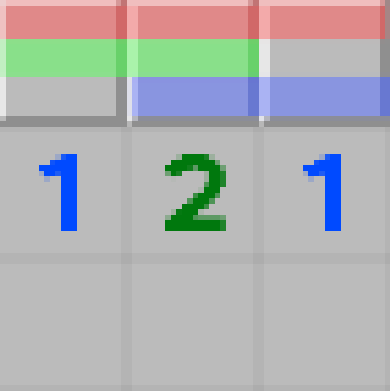
\includegraphics[scale=0.25]{images/uroven2-2.png}
        \caption{Situace z dvěmi bombami}
        \label{fig:situace_u2_dva}
    \end{subfigure}
    \begin{subfigure}[b]{0.3\textwidth}
        \centering
        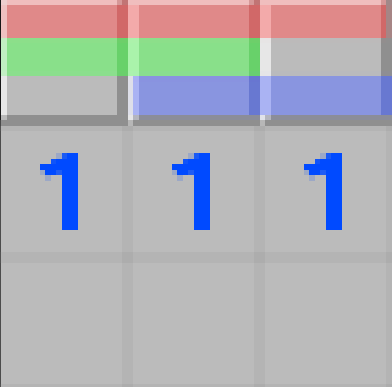
\includegraphics[scale=0.25]{images/uroven2-1.png}
        \caption{Situace s jednou bombou}
        \label{fig:situace_u2_jedna}
    \end{subfigure}
    \caption{Situace řešitelné 2. úrovní automatu}
    \label{fig:sitauce_u2}
\end{figure*}

\section{Automat}
Automat, který dokáže řešit hru, je hlavní odlišení projektu Autosweeper od původní hry. Algoritmus dostane jako vstupní data
herní pole a jeho stav přesně tak, jak je zobrazeno na obrazovce. Neví tedy, kde miny opravdu jsou a kde ne. Cíl automatu je
poté navrhnout možné tahy, které si myslí, že jsou bezpečné. Je strukturovaný do tří úrovní, každá se snaží najít možné tahy,
pokud žádný nenajde, je spuštěna další úroveň.

\subsection{První tah}
První tah hry se liší od ostatních tím, že je jisté, že není možné vydedukovat pozici žádné bomby. Nejdříve je nutné vyřešit
problém s rozlišením "začínající" hry od ostatních. Hra je pro automat začínající, jestliže se na herním poli nevyskytuje
žádná políčka s číslem (počtem \\bomb v okolí) 0 a počet odehraných tahů je méně než čtyři.

V této situaci automat odkrývá políčka v rozích, protože vzhledem k počtu okolních políček je nejvíce pravděpodobné, že stav
políčka nebude možné vydedukovat. \cite{bercerra2015} Pravděpodobnost výhry se tím sice nezmění, ale algoritmus alespoň neplýtvá
čas řešením hry ve které bude muset hádat.

\subsection{První úroveň}
První úroveň automatu je algoritmus, který se dívá na stav každého odhaleného políčka a pokud se jeho číslo schoduje s počtem
neodhalených sousedů (8 sousedících políček) tak všechny sousedy označí jako bomby. Po zkontrolování celého pole jde zpátky na
začátek a prochází celé pole znovu. Hledá políčka u kterých se jejich číslo schoduje s počtem nalezených bomb, jestliže taková
situace nastane, jsou odhaleni všichni sousedi, kteří nebyli označeni jako bomba.

Komplexitu prvního stupně odhaduji na \\$O(8n)$. V praxi je ale vyhodnocování pole mnohem rychlejší vzhledem k počtu políček s číslem 0, které jsou pro výpočet zanedbatelné.

\begin{figure*}[ht!]
    \centering
    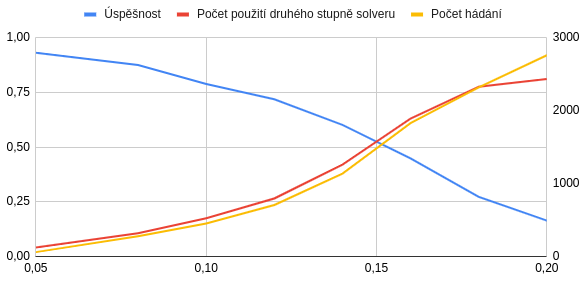
\includegraphics[scale=0.60]{images/uspesnost.png}
    \caption{Úspěšnost automatu na poli 20x20 pro různé obtížnosti hry}
    \label{fig:uspesnost}
\end{figure*}

\subsection{Druhá úroveň}
Druhá úroveň je spuštěna v případě, že první úroveň nic nenašla. Pracuje již s označenými bombami a snaží se vyřešit další
situace za pomocí spojení více neznámých políček do množin, neboli "kyblíků". Na obrázcích (\ref{fig:sitauce_u2}) lze vidět jakou
strukturu kyblíky mají. Červenou je označen kyblík prostřední číslice, levá číslice má zelený a pravá modrý. Červený kyblík je
hlavní, jelikož to je kyblík políčka, které se snažíme vyřešit. Všechny ostatní kyblíky musí být podmnožinou hlavního, abychom je
mohli od sebe odčítat. Tato limitace omezuje druhou úroveň na řešení situací 3x3. První úroveň tomuto velmi pomáhá, protože může
působení druhé úrovně rozšířit tím, že označí už odhalené bomby a zvýší tak šanci, že nějaký kyblík nebude přesahovat ven z
hlavního.

Poté co byli nalezeny všechny kyblíky a bylo zajištěno, že se mezi nimi nenachází žádné duplikáty, je potřeba vyřešit průniky
dvou, či více kyblíků. V situaci na obrázcích (\ref{fig:sitauce_u2}) se nachází jeden průnik a to mezi zeleným a modrým kyblíkem.
Algoritmus se nejdřív snaží najít jakékoliv políčko, které je ve více než jednom kyblíku. Pokud nějaké políčko najde, snaží se
dohledat celý průnik. Každý průnik poté zkusí vyhodnotit tím, že odečte očekávaný počet bomb v průniku od všech pronikajících
kyblíků včetně hlavního kyblíku. Jestliže součet vypočítaných hodnot je roven $0$, pak je v průniku bomba a jakékoliv jiné
políčko algoritmus považuje za bezpečné. Když součet naopak $0$ roven není, je třeba průnik ze všech pod-kyblíků odstranit bez
odčítání z celkového počtu bomb. Tedy průnik obsahuje všechny miny v hlavním kyblíku, jestliže následující rovnost platí:
\begin{equation*}
\sum_{x \in K} |x-\min K| = 0
\end{equation*}
Kde $K$ je množina počtů bomb všech pronikajících kyblíků a hlavního kyblíku.

Po ošetření průniků algoritmus odčítá všechny pod-kyblíky od hlavního (tzn. odstranit všechny políčka pod-kyblíku z hlavního
kyblíku a odečtení počtu bomb). Všechny zbylé políčka v hlavním kyblíku lze považovat za bezpečné za podmínky, že počet bomb se
rovná $0$. Při nerovnosti algoritmus výpočet zahodí a přechází na další políčko.


\subsection{Třetí úroveň}
Aby automat vždy navrhl nějaké políčko, je potřeba třetí úroveň. Tato úroveň se nesnaží vydedukovat bezpečné políčka, ale spočítá
jednoduchou pravděpodobnost bomby na každém políčku. Vzhledem k tomu, že výpočet pravé pravděpodobnosti výskytu bomby na políčku
je stejně těžký úkol jako samotné řešení, není pravděpodobnost z výpočtu pravdivá, ale jaksi orientační. Každé políčko dostane
pravděpodobnost jednoduchým výpočtem, který se provede pro každé odhalené políčko: $p = \frac{c}{n}$, kde $c$ je číslo na
odhaleném políčku a $n$ je počet neodhalených sousedů. V případě, že na jedno políčko bude víc pravděpodobností, algoritmus vybere
nejvyšší. Po výpočtu všech pravděpodobností algoritmus vybere políčko s nejmenší pravděpodobností výskytu bomby.


\subsection{Limity}
Autosweeper nedokáže vyřešit všechny Minesweeper hry. Řešení těchto her je těžký matematický problém, Richard Kaye ve své studii
nazvané "Minesweeper is NP-Complete" \\argumentuje mnoha způsoby, že Minesweeper problém je NP-úplný \cite{Kaye2000}. To by
znamenalo, že je jeden z nejtěžších matematických problémů a jeho komplexita by byla stejná jako ta známého problému s obchodním
cestujícím \cite{wiki_tsp}. \\Vždy úspěšný automat je hned vyloučen při prvním tahu, kdy je vždy možné narazit na minu. Záleží
tedy na implementaci hry, jestli první tah udělá zaručeně dobrým, nebo jestli herní pole bude už přegenerované (způsob používán
Autosweeperem).

Aby se dala kvantifikovat úspěšnost Autosweeperu, byl spuštěn vždy na 1000 her pro různé nastavení a z výsledků se vytvořil graf
(obrázek \ref{fig:uspesnost}). Na grafu lze vidět, že automat má při jednoduché hře (pravděpodobnost výskytu min $0,05$) vysokou
úspěšnost a zároveň řeší většinu tahů jen pomocí prvního stupně. Při pravděpodobnosti $0,15$ je automat úspěšný jen v polovině
her. Tyto hry jsou těžké i pro lidské hráče. Při pravděpodobnosti $0,20$, tedy každé páté políčko je v průměru mina, automatu
selhává i druhý stupeň algoritmizace a je vidět, že automat ve většině případech hádá.

